\documentclass[border=10pt]{standalone}

\usepackage{tikz}
\usepackage{tikzsymbols}
\usetikzlibrary{calc,patterns,shapes.geometric}

\def\centerarc[#1](#2)(#3:#4:#5){\draw[#1] ($(#2)+({#5*cos(#3)},{#5*sin(#3)})$) arc (#3:#4:#5);}

\begin{document}
	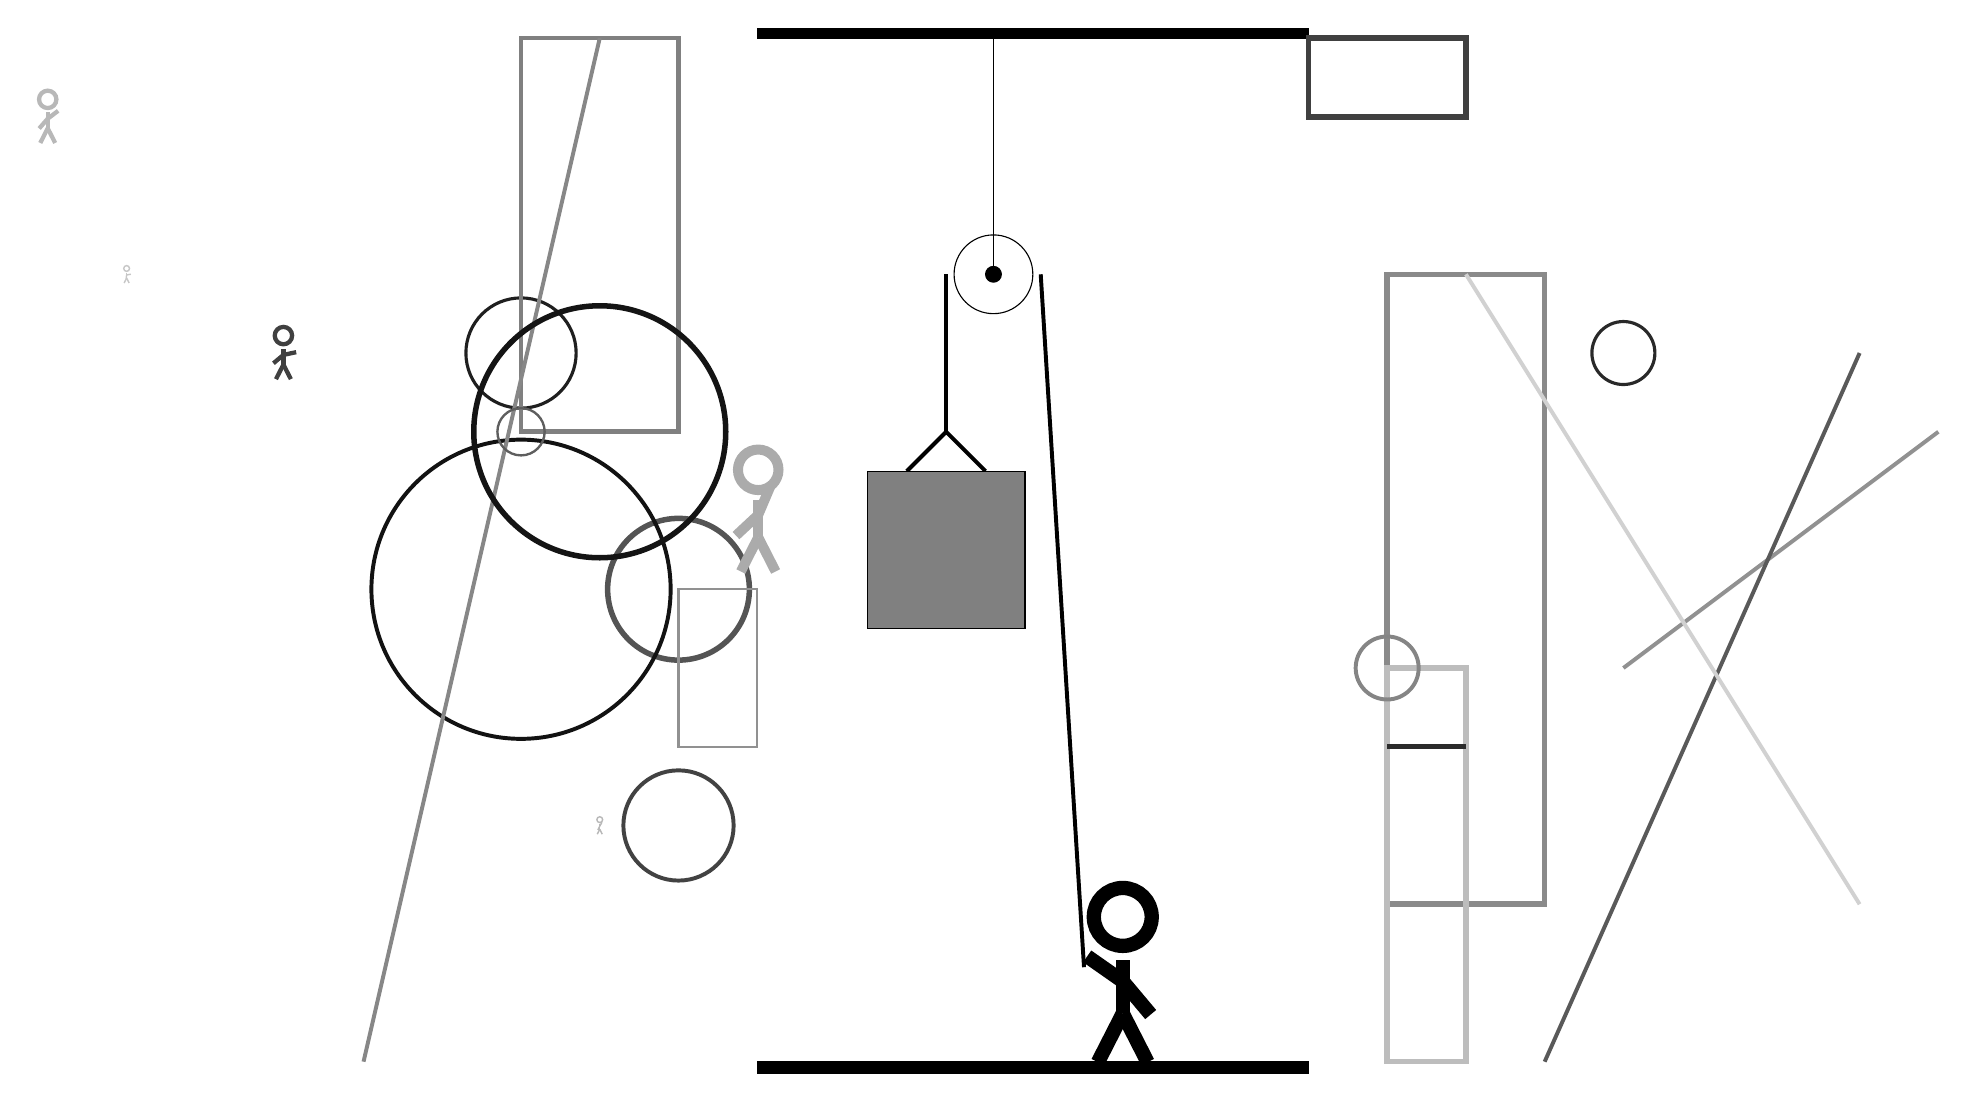
\begin{tikzpicture}
		%%%%% START %%%%%
		
		\draw[fill=black] (-2, 10) rectangle (5, 10.125);
		
		\node[line width=0.3mm, color=black!28] at (-4, 0) {\Strichmaxerl[1][64][60]};
		
		\draw[line width=0.5mm, color=black!43](9, 2) -- (13, 5);
		\draw [line width=0.7mm, color=black!67](-3, 3) circle (0.9);
		\draw [line width=0.5mm, color=black!93](-5, 3) circle (1.9);
		
		\draw[line width=0.7mm, color=black!46] (6, -1) rectangle (8, 7);
		\draw[line width=0.5mm, color=black!65](8, -3) -- (12, 6);
		\draw [line width=0.4mm, color=black!88](-5, 6) circle (0.7);
		
		\draw[line width=0.7mm, color=black!26] (6, 2) rectangle (7, -3);
		\draw [line width=0.5mm, color=black!74](-3, 0) circle (0.7);
		\draw[line width=0.6mm, color=black!50] (-3, 10) rectangle (-5, 5);
		\draw[line width=0.3mm, color=black!43] (-2, 3) rectangle (-3, 1);
		\node[line width=0.5mm, color=black!28] at (-11, 9) {\Strichmaxerl[3][49][37]};
		\draw[line width=0.5mm, color=black!47](-7, -3) -- (-4, 10);
		
		\node[line width=0.7mm, color=black!75] at (-8, 6) {\Strichmaxerl[3][40][12]};
		\draw[line width=0.7mm, color=black!75] (5, 9) rectangle (7, 10);
		\node[line width=0.5mm, color=black!22] at (-10, 7) {\Strichmaxerl[1][84][9]};
		
		\draw [line width=0.3mm, color=black!63](-5, 5) circle (0.3);
		\draw [line width=0.4mm, color=black!84](9, 6) circle (0.4);
		\draw[line width=0.5mm, color=black!18](7, 7) -- (12, -1);
		\draw [line width=0.5mm, color=black!48](6, 2) circle (0.4);
		\node[line width=0.5mm, color=black!33] at (-2, 4) {\Strichmaxerl[7][43][67]};
		\draw[line width=0.6mm, color=black!83] (6, 1) rectangle (7, 1);
		
		\draw [line width=0.7mm, color=black!92](-4, 5) circle (1.6);
		
		\draw (1, 7) circle (0.5);
		\draw[fill=black] (1, 7) circle (0.1);
		\draw (1, 10) -- (1, 7);
		
		\draw[line width=0.5mm] (-0.1, 4.5) -- (0.4, 5.0) -- (0.9, 4.5);
		\draw[fill=black!50] (-0.6, 4.5) rectangle (1.4, 2.5);
		
		\draw[line width=0.5mm] (0.4, 7) -- (0.4, 5.0);
		\centerarc[line width=0.5mm](1, 7)(0:180:0.6);
		\draw[line width=0.5mm](1.6, 7) -- (2.15, -1.8);
		
		\node at (2.6, -1.9) {\Strichmaxerl[10][-35][-50]};
		
		\draw[fill=black] (-2, -3) rectangle (5, -3.15);
		
		%%%%% END %%%%%
	\end{tikzpicture}
\end{document}